\documentclass{article}

\usepackage[utf8]{inputenc}
% \usepackage[latin1]{inputenc}
\usepackage[ngerman,naustrian]{babel}
\usepackage{lmodern}
\usepackage[T1]{fontenc}
\usepackage{ulem}
\usepackage{here}
\usepackage[pdftex]{graphicx}
\usepackage{amsthm}
\usepackage{gensymb}
\usepackage{fancyhdr}
\usepackage[left=20mm,top=25mm,bottom=25mm,right=20mm,headheight=15mm,headsep=10mm,footskip=10mm]{geometry}
\usepackage{longtable}
\usepackage{hhline}
\usepackage[table]{xcolor}
\usepackage{amsfonts}
\usepackage{amssymb}
\usepackage{amsmath}
\usepackage{mathcomp}
\usepackage{tabularx}
\usepackage{multicol}
\usepackage{graphicx}
\renewcommand{\familydefault}{\sfdefault}
		% \sffamily


\begin{document}

%\pagestyle{empty}
\begin{titlepage}
	\begin{center}
		{\large{FH OÖ - Hagenberg \\ embedded systems design}\\\vspace*{4cm}}
		\small{RTO1 UE}\\
		\textbf{WS 2020}\\\vspace*{2cm}
		\Huge{\textbf{Protokoll}}\\\vspace*{1cm}
		\huge{Übung\,1: Vorversion von Betriebssystemen\\ \large{kooperative Weitergabe an Tasks } } \vspace*{90mm}
		
		\small{Simon Steindl  S2010567025	\\
		Florian Hinterleitner S2010567014	\\
		}
	\end{center}
\end{titlepage}

% \tableofcontents
% \newpage
% \setcounter{page}{18}
% \setcounter{section}{3}
 
\section{Übungsaufgabe A – Erstellung einer Debug-Unit}
% screenshots
% Timing-tabelle

\subsection{Ergebnisse}
\subsection{Laufzeit jedes Tasks}
\subsection{ Screenshots der Messungen }
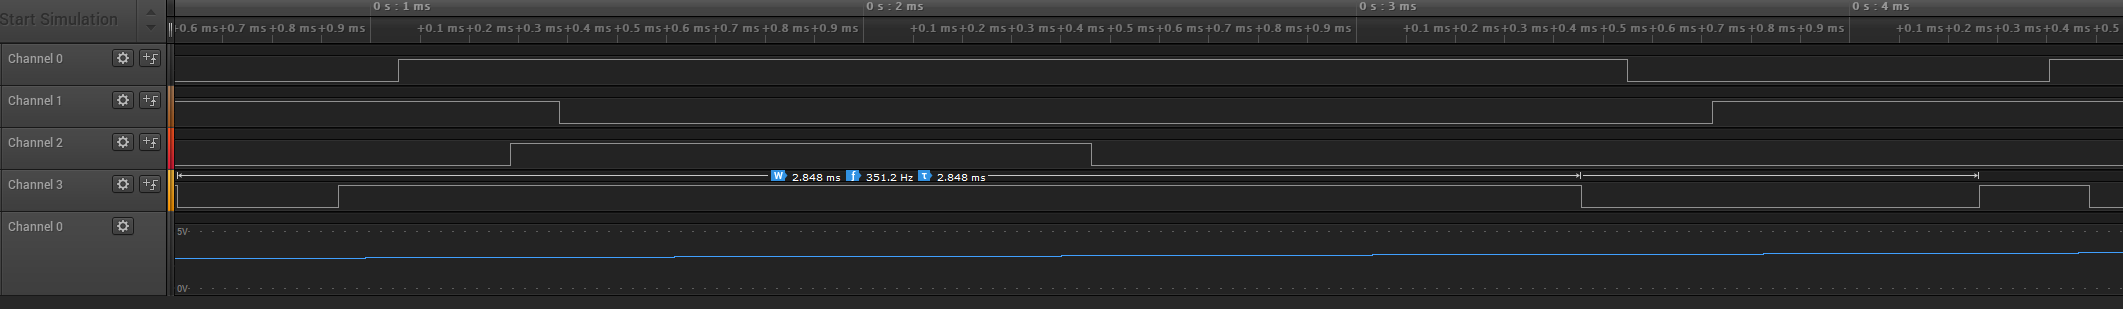
\includegraphics[width=.8\textwidth]{Saleae_nonense}
\subsection{Overhead (Zyklen, µs) der Messung}

\section{Übungsaufgabe B – Reaktionsgeschwindigkeit bei Superloops}
\ldots

\end{document} 